\documentclass[12pt,a4paper,notitlepage]{article}

\usepackage[utf8]{inputenc}

\usepackage[francais]{babel}\usepackage[T1]{fontenc}
\usepackage[cyr]{aeguill}
\usepackage{lmodern}
\usepackage{color}
\usepackage{boites}
\usepackage{caption}
\usepackage{fancybox}
\usepackage{listings}
\usepackage{multicol}
\usepackage[table]{xcolor}

\usepackage[T1]{fontenc}
\usepackage[scaled]{helvet}
\renewcommand*\familydefault{\sfdefault}

%\lstset{language=bash, basicstyle=\footnotesize, frame=shadowbox, rulesepcolor=\color{gris}, captionpos=b}

  \lstset{
         basicstyle=\footnotesize\ttfamily, % Standardschrift
         %numbers=left,               % Ort der Zeilennummern
         numberstyle=\tiny,          % Stil der Zeilennummern
         %stepnumber=2,               % Abstand zwischen den Zeilennummern
         numbersep=5pt,              % Abstand der Nummern zum Text
         tabsize=2,                  % Groesse von Tabs
         extendedchars=true,         %
         breaklines=true,            % Zeilen werden Umgebrochen
         keywordstyle=\color{red},
                frame=b,         
         keywordstyle=[1]{\itshape}{//},    % Stil der Keywords
         stringstyle=\color{white}\ttfamily, % Farbe der String
         showspaces=false,           % Leerzeichen anzeigen ?
         showtabs=false,             % Tabs anzeigen ?
         xleftmargin=5pt,
         framexleftmargin=1pt,
         framexrightmargin=5pt,
         %numbers=left,
         frame=toplines,
         framextopmargin=3pt,
       %  framexleftmargin=8pt,
         numberblanklines=false,
         %morecomment=[s][marron]{/*}{*/},
         %moredelim=*[s][\color{blue}]{/*}{*/}
         %morecomment=[s][marron]{/*-}{*/}},         
         framexbottommargin=5pt,
         captionpos=b,
         %backgroundcolor=\color{lightgray},
         showstringspaces=false      % Leerzeichen in Strings anzeigen ? 
 }

\DeclareCaptionFont{white}{\color{white}}
\DeclareCaptionFormat{listing}{\colorbox[cmyk]{0.43, 0.35, 0.35,0.01}{\parbox{\textwidth}{\hspace{10pt}#1#2#3}}}
\captionsetup[lstlisting]{format=listing,labelfont=white,textfont=white, singlelinecheck=false, margin=0pt, font={bf,footnotesize}}

\definecolor{gris}{gray}{0.75}
\definecolor{bleup}{HTML}{258EE9}


%\renewcommand*\familydefault{\ttdefault} %% Only if the base font of the document is to be typewriter style
%\renewcommand{\rmdefault}{ptm}


\usepackage[
   pdfauthor={Ludovic Terrier & Arnaud Goulut},
   pdftitle={RE12 - TP6},
   ]{hyperref}
   
   
\usepackage[pdftex]{graphicx}

%\usepackage{titlesec}
%\titleformat{\section}[frame] {\normalfont} {\filright
%\footnotesize
%\enspace\textbf{\thesection}\enspace} {8pt} {\Large\bfseries\filcenter}

%% Je contrôle la taille de ma zone imprimée...
\usepackage{anysize}
%% ...en définissants les marges {gauche}{droite}{haute}{basse}
\marginsize{25mm}{15mm}{10mm}{15mm}

\begin{document}

\title{Gestion de réseau par SNMP}
\author{Ludovic Terrier et Arnaud Goulut}
\date{Juin 2010}
\maketitle


%\tableofcontents

\thispagestyle{empty}


 
%%%%%%%%%%%%%%%%%%%%%%%%%%%%%%%%%%% 1ère partie
\section{Configuration et prise en main de l'agent SNMP}
\subsection{Installation d'un agent snmp}
L'agent \texttt{net-snmp} était déjà installé lorsque nous avons pris possession de la salle de TP, il nous a donc simplement fallut éditer le fichier de configuration \textit{snmpd.conf} pour le faire fonctionner comme nous le désirions :
\begin{lstlisting}[title=snmpd.conf]
rocommunity publicB3
rwcommunity privateB3
\end{lstlisting}

Nous avons fait au plus simple, ainsi la communauté \textbf{publicB3} est autorisée a consulter les informations contenues dans la \textit{MIB}\footnote{Management Information Base}, alors que \textbf{privateB3} peut lire, mais aussi écrire dans cette même base.

\subsection{Ligne de commande}
Afin de consulter la MIB disponible sur notre machine, il nous a fallut installer le programme \texttt{net-snmp-utils} via les dépôts Fedora (\texttt{yum install}). Nous avons ensuite pu tester les différentes commandes disponibles :\\

\begin{itemize}
\item \texttt{snmpget} : permet de récupérer les informations d'une instance précise.
\item \texttt{snmpgetnext} : permet de récupérer les informations de l'instance disponible suivante.
\item \texttt{snmpwalk} : permet de récupérer les informations d'un sous-arbre donné.
\item \texttt{snmptable} : permet d'afficher une table. \\
\end{itemize}

Exemple d'utilisation de la commande \texttt{snmptable}, pour afficher l'ensemble des informations contenu dans la table des connections TCP (objet 1.3.6.1.2.1.6.13) :
 \lstset{
         basicstyle=\scriptsize\ttfamily,
         }
\begin{lstlisting}[title=snmptable]
root@pc05-d202 snmp]# snmptable -v 2c -c publicB3 127.0.0.1 1.3.6.1.2.1.6.13
SNMP table: TCP-MIB::tcpConnTable

tcpConnLocalAddress tcpConnLocalPort tcpConnRemAddress tcpConnRemPort
0.0.0.0              111           0.0.0.0              0
127.0.0.1               25           0.0.0.0              0
127.0.0.1              199           0.0.0.0              0
192.168.3.1            39628     188.165.75.23             22
\end{lstlisting}



\subsection{MibBrowser}
SIP peut envoyer deux types de messages (textuels basés sur HTTP 1.0) :


Passons maintenant au détail d'un paquet SIP :

\paragraph{} Revenons sur le paramètre \textit{Cseq} contenu dans l'en-tête, celui-ci est un indentifiant d'échanges liant les requêtes aux réponses. Il est incrémenté à chaque nouvelle requête.

\section{Surveillance des équipements réseau et alarmes}
\subsection{Configuration équipements}
Pour les besoins du

\subsection{Perte de connectivité}
Pour le hardphone, on utili

\subsection{Le démon snmptrapd}
dfdfklsjfkj

\section{Prise en main d'une console de supervision}
\subsection{Installation de ZenOSS}
Ce fichier définit l'ensemble des options du protocole SIP qui seront utilisées lorsque notre serveur de téléphonie sera en fonctionnement. \\
\begin{lstlisting}[title=sip.conf v1]
[user1]
username=user1
\end{lstlisting}

\subsection{Parcours des fonctionnalités}

Dans \textit{Asterisk}, les extensions définissent une série d'étapes uniques qui vont être déroulées au cours d'un appel. Pour définir une extension, on utilise la forme : \\

%\paragraph{}Voici le schéma décrivant l'infrastructure du réseau que nous désirons obtenir :
%\clearpage%
%\begin{figure}[!h]
%\begin{center}
%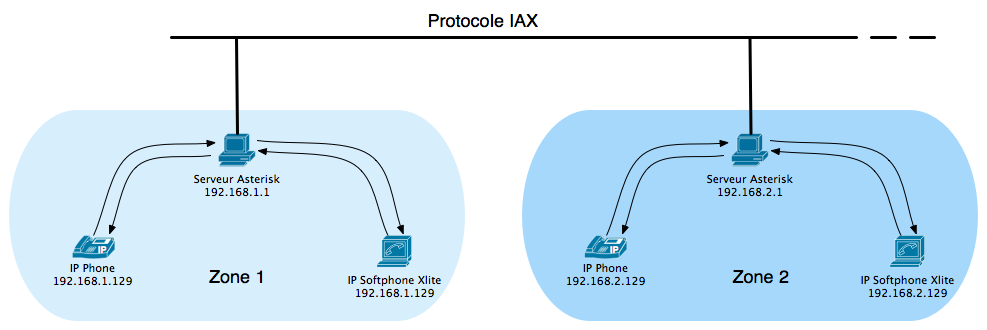
\includegraphics[height=5cm]{structure_reseau_IAX}
%\caption{Structure du réseau}
%\label{fig:da}
%\end{center}
%\end{figure}
\end{document}